{
\usebackgroundtemplate{  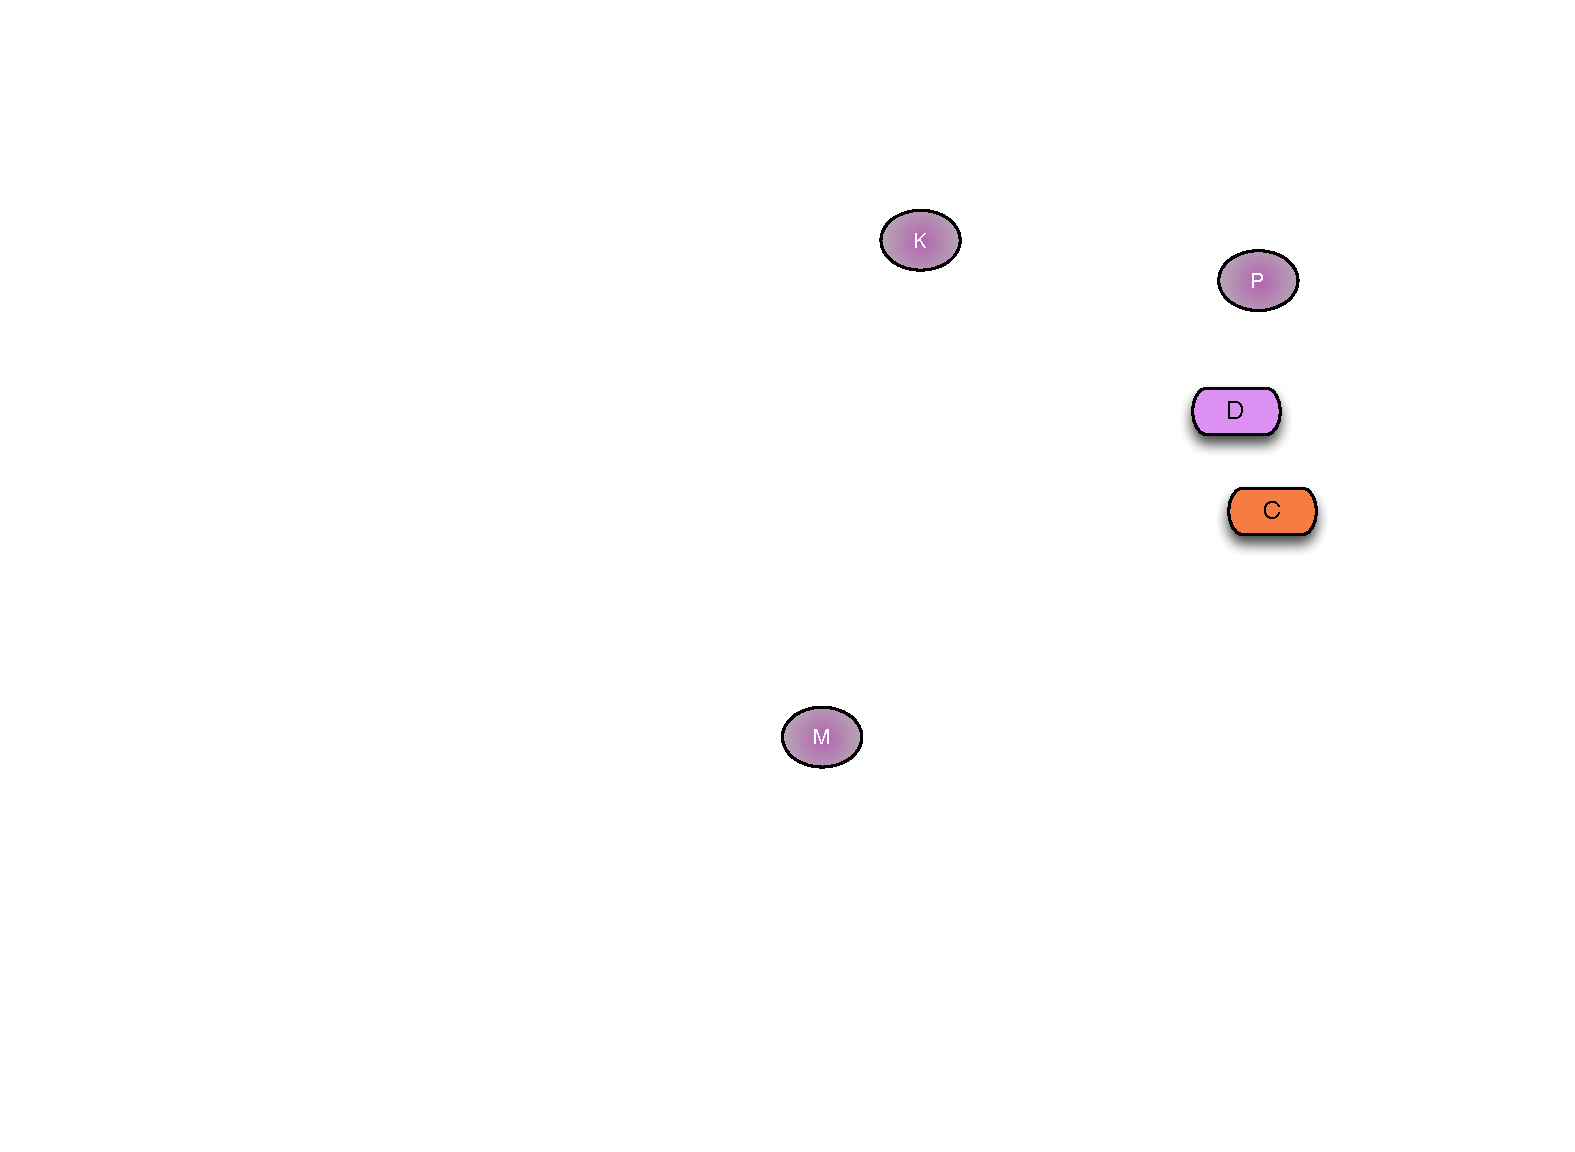
\includegraphics[width=\paperwidth]{../figures/progmodel/01-objects-for-algo.pdf} }
\begin{frame}[t]
  \frametitle{Express parallel algo independent of processors}
  Use units natural to domain
  \begin{itemize}
    \item matrix block
    \item tile of an image
    \item chunk of a mesh
    \item volume of simulation space
    \item partition of a graph, tree or other data structures
  \end{itemize}
\end{frame}
}

\begin{frame}
  \frametitle{Data decomposition: via an object collection}
  \begin{figure}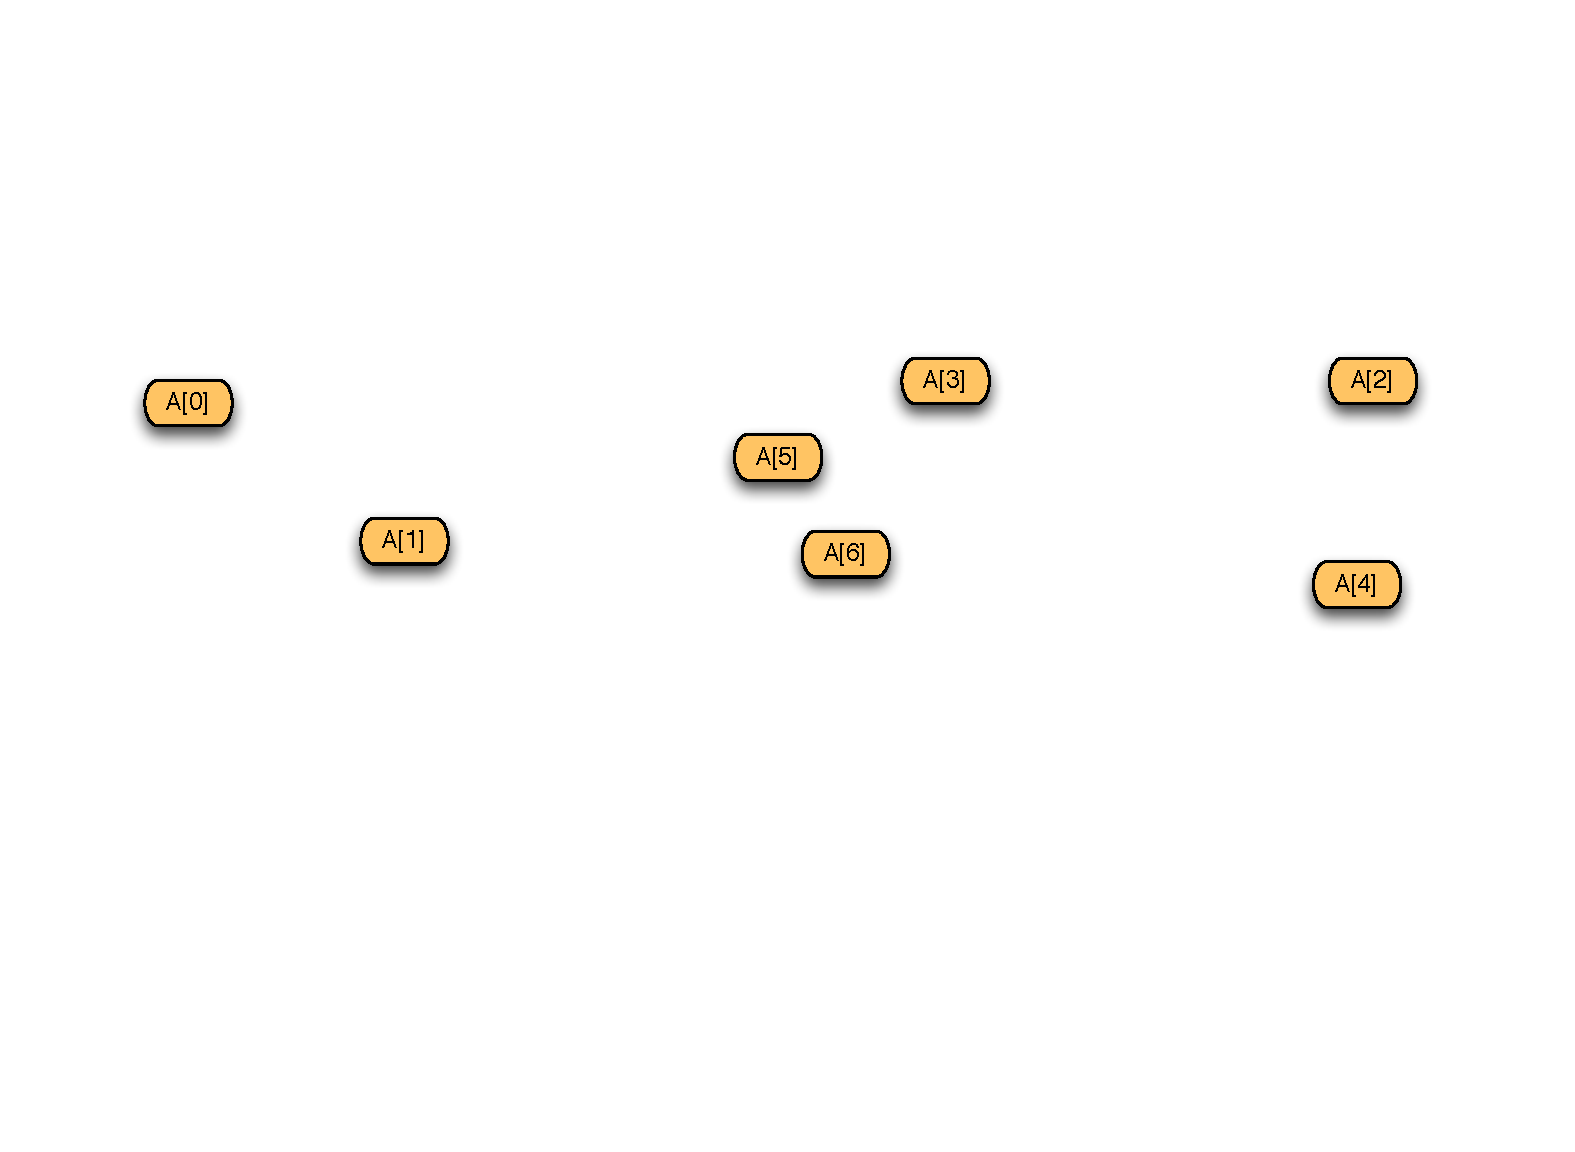
\includegraphics[width=0.9\textwidth]{../figures/progmodel/02-data-decomp-via-arrays.pdf}\end{figure}
\end{frame}


\begin{frame}
  \frametitle{Multiple data parallel collections}
  \begin{figure}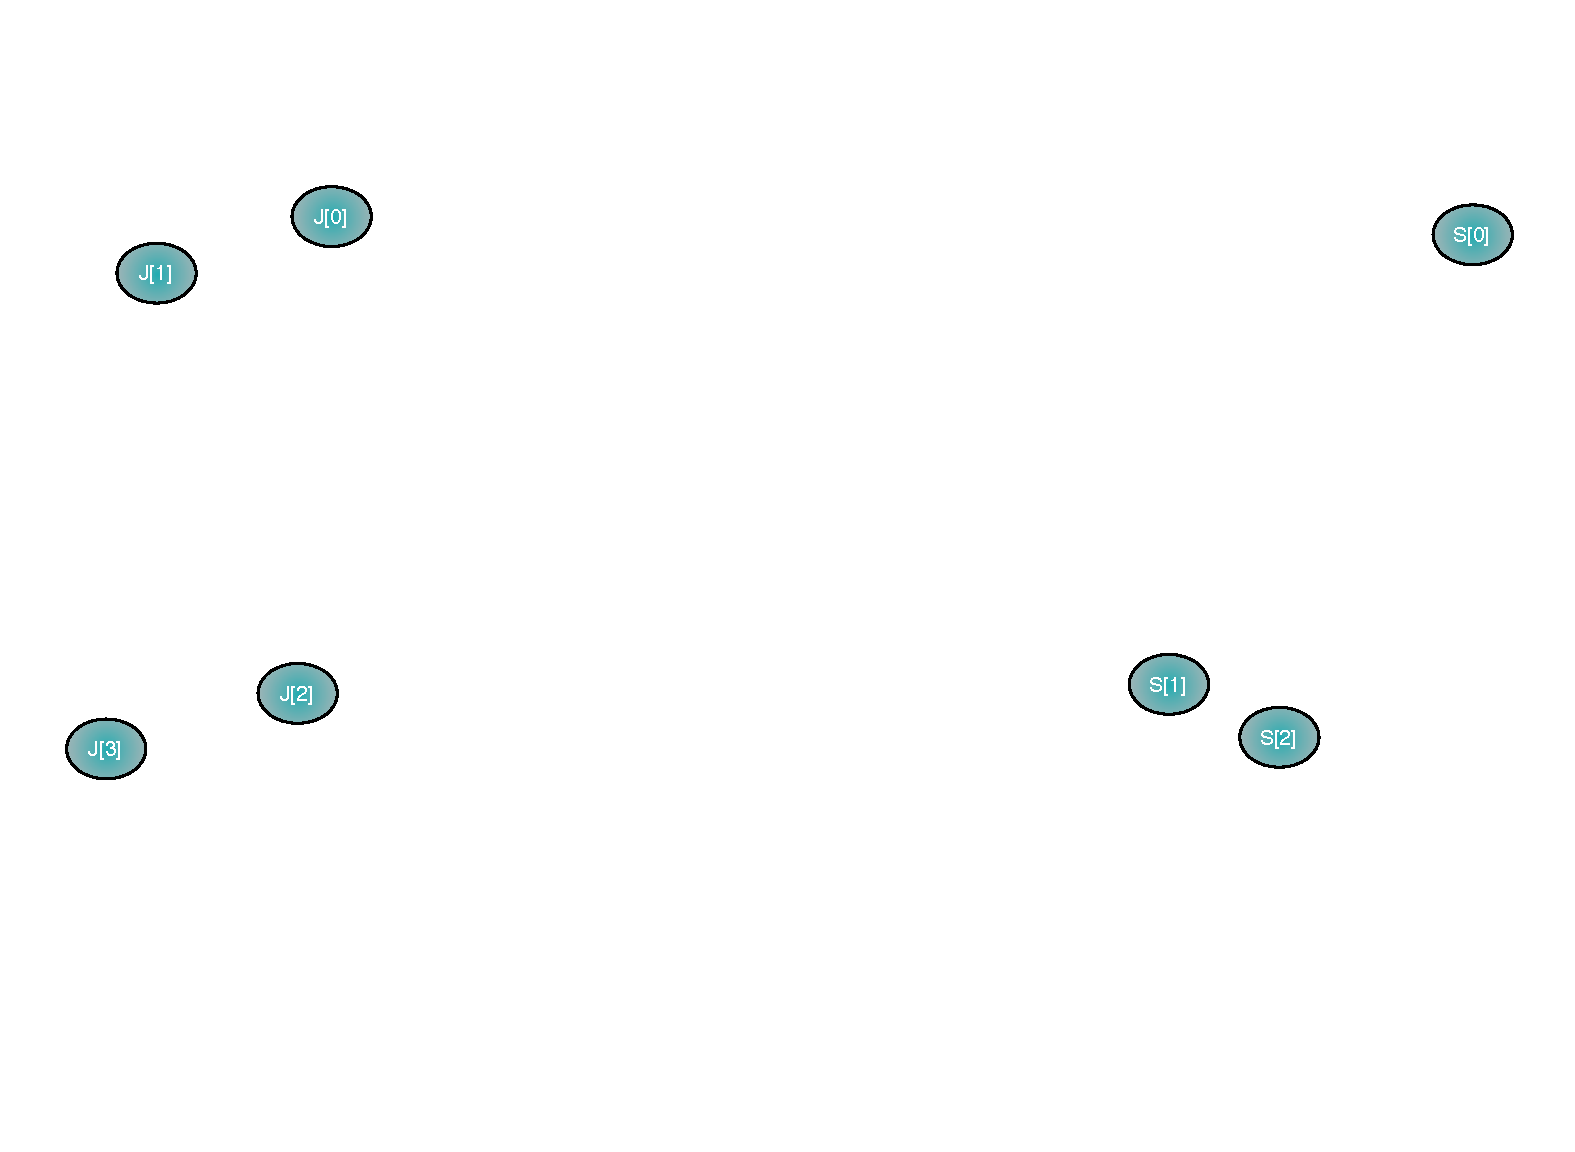
\includegraphics[width=0.9\textwidth]{../figures/progmodel/03-many-data-parallel-arrays.pdf}\end{figure}
\end{frame}


\begin{frame}
    \frametitle{Work decomposition: also via objects / collections}
  \begin{figure}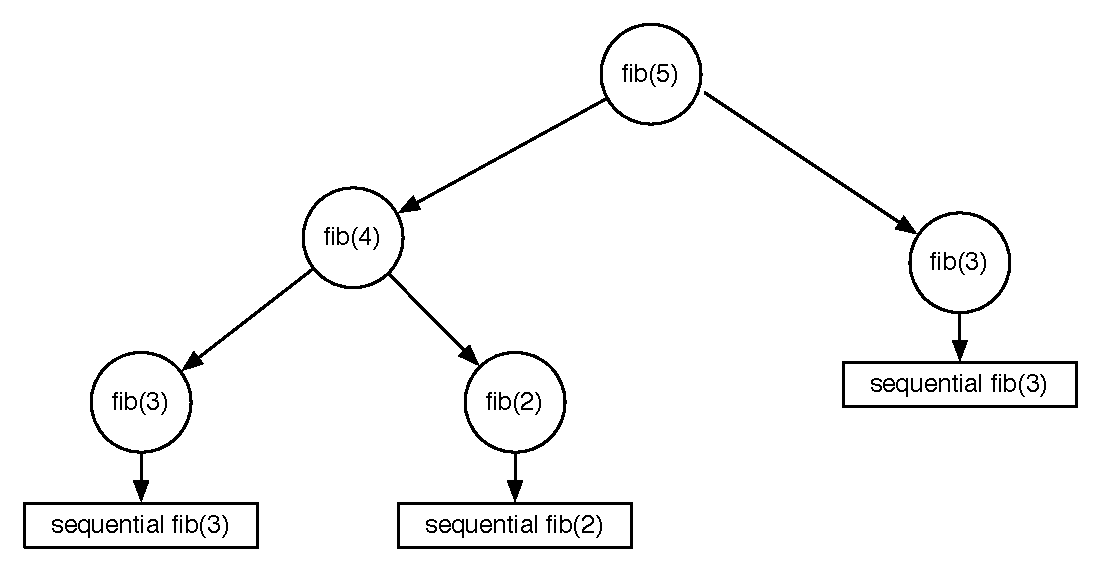
\includegraphics[width=0.9\textwidth]{../figures/tree-threshold.pdf}\end{figure}
\end{frame}


\begin{frame}
  \frametitle{Functional decomposition: via multiple classes}
  \begin{figure}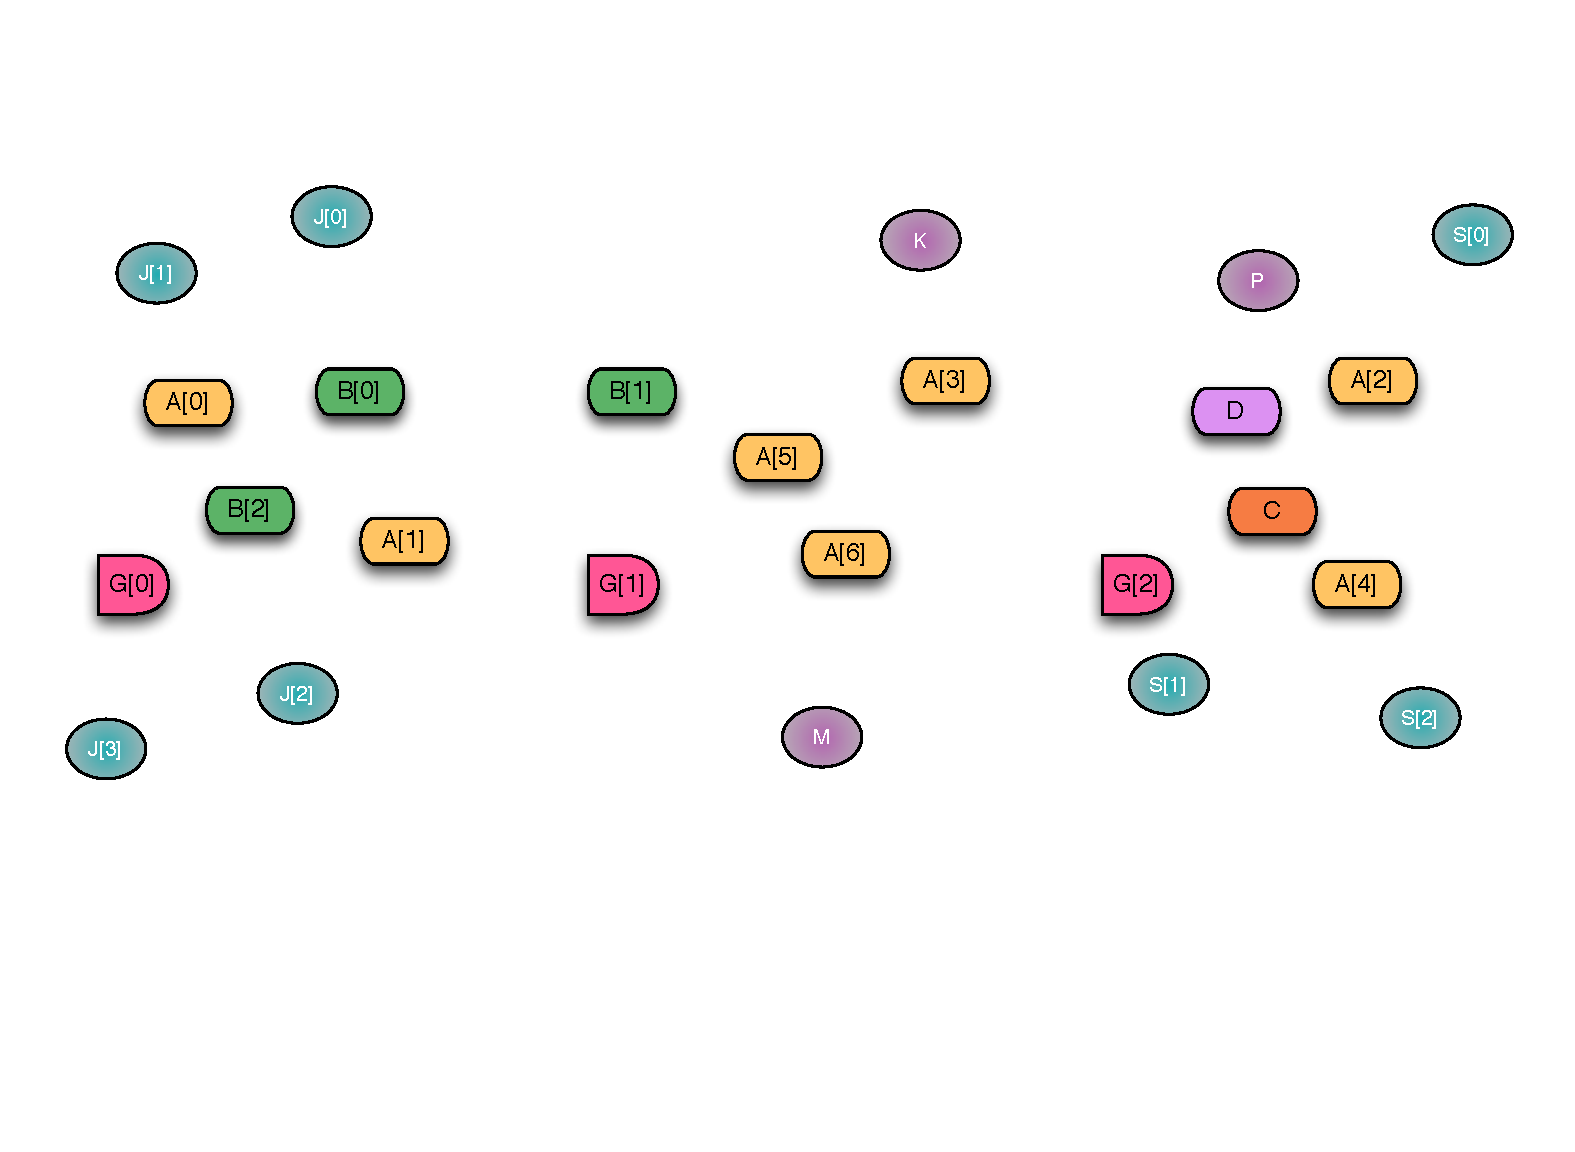
\includegraphics[width=0.9\textwidth]{../figures/progmodel/04-func-decomp-via-classes.pdf}\end{figure}
\end{frame}


\begin{frame}
  \frametitle{App logic: via classes and objects collections}
  \begin{figure}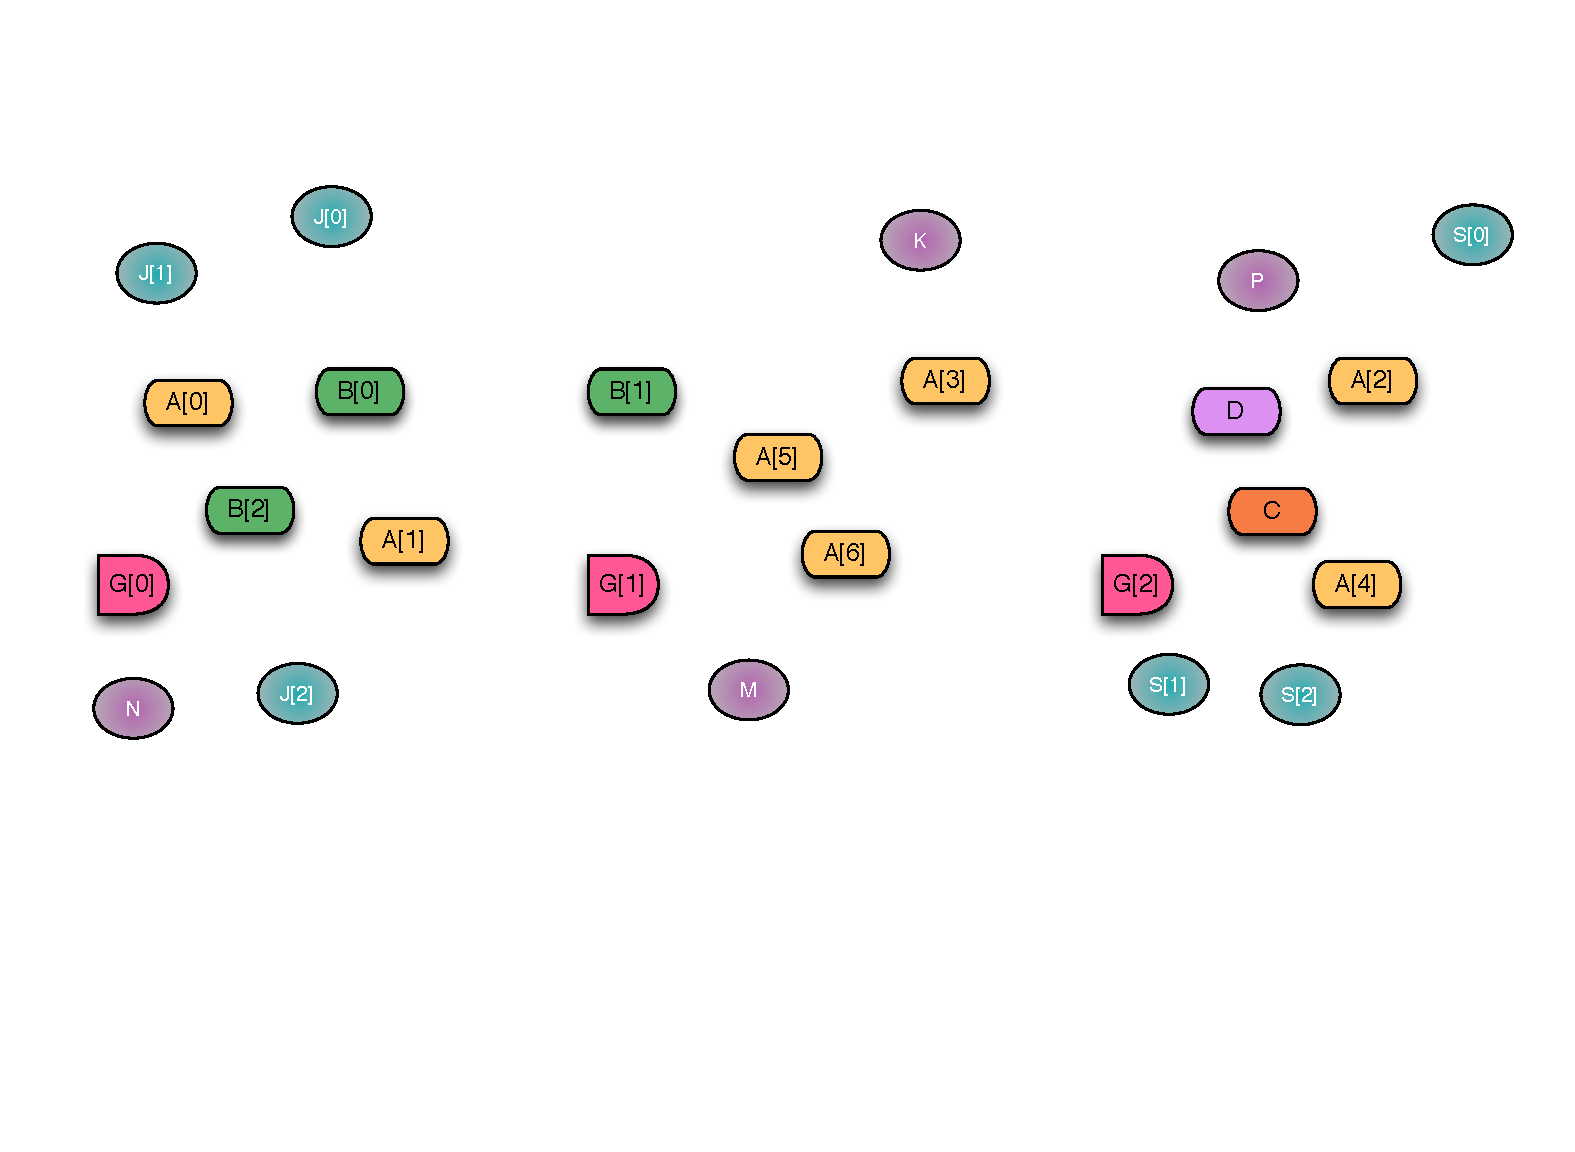
\includegraphics[width=0.9\textwidth]{../figures/progmodel/05-parallelism-via-obj-collections.pdf}\end{figure}
\end{frame}


\begin{frame}
  \frametitle{
    \only<1>{Parallelism requires distributing objects across processors}
    \only<2>{However, do not burden programmer with this view}
  }
  \begin{figure}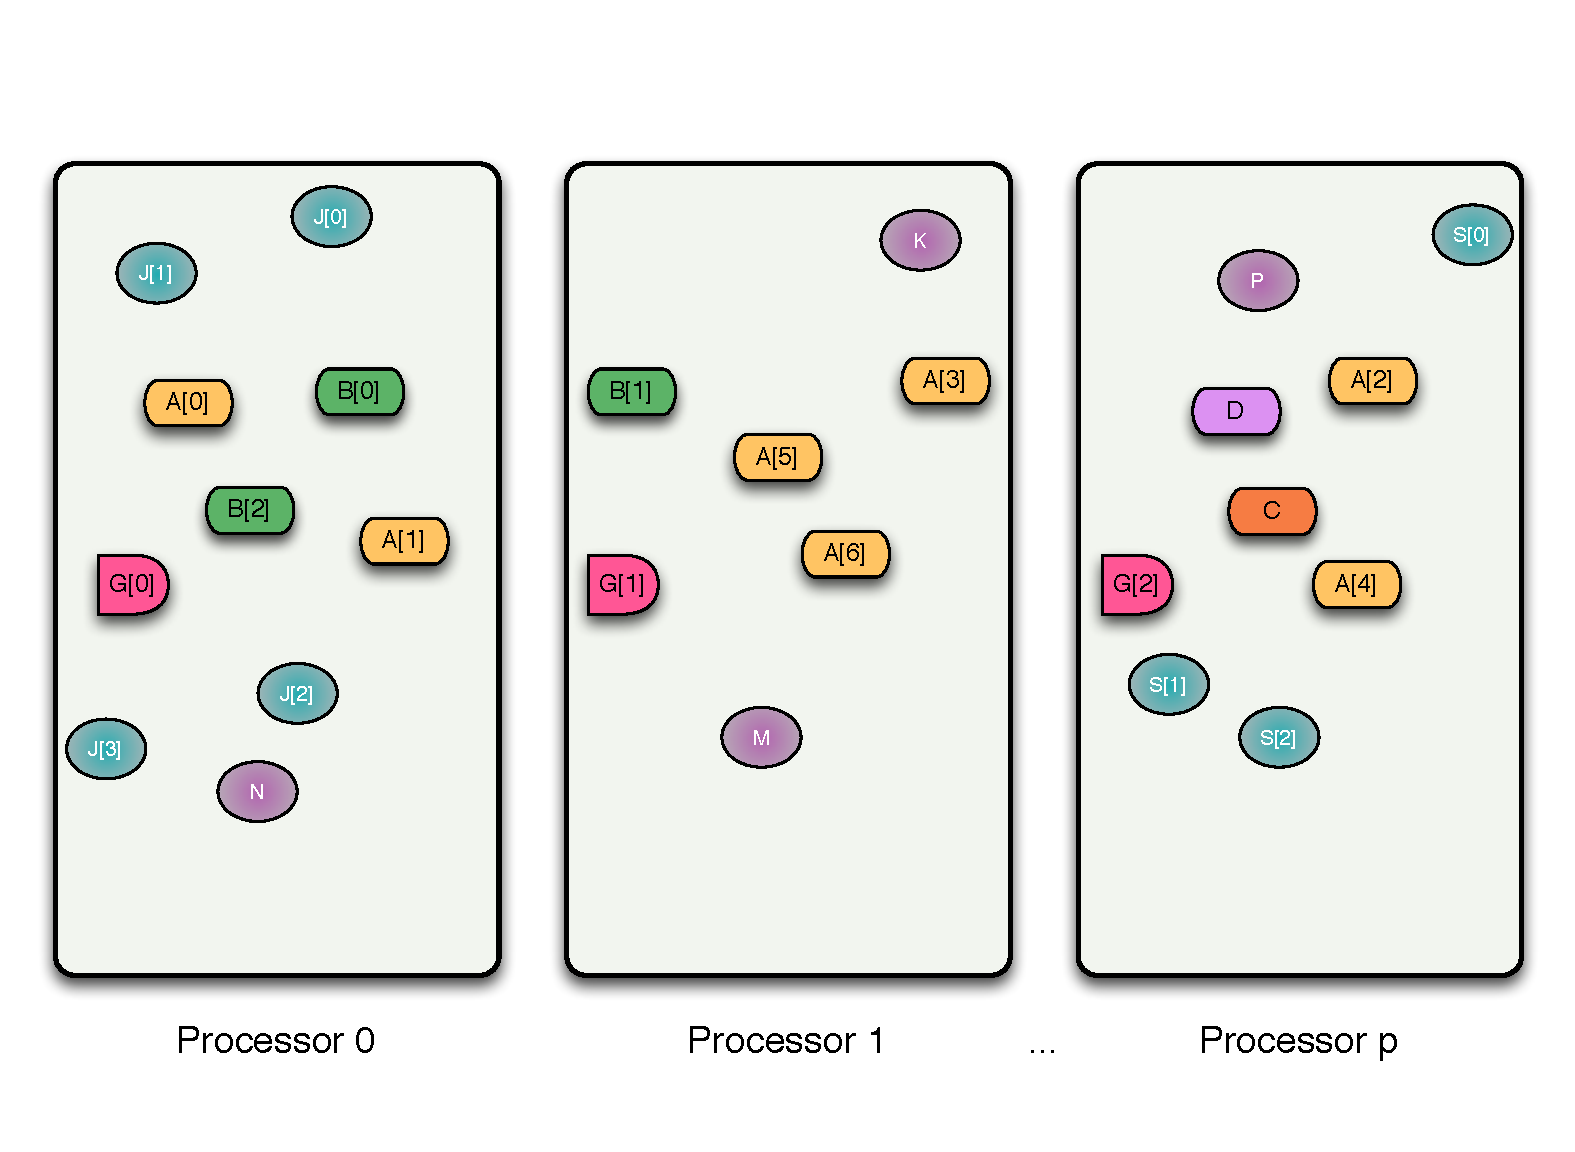
\includegraphics[width=0.9\textwidth]{../figures/progmodel/06-objects-sys-view.pdf}\end{figure}
\end{frame}


\begin{frame}
  \frametitle{
    \only<1>{Elevate some objects to global visibility}
    \only<3>{Globally visible objects = chares}
    \only<4>{Globally visible object collections = chare arrays}
  }
  \begin{figure}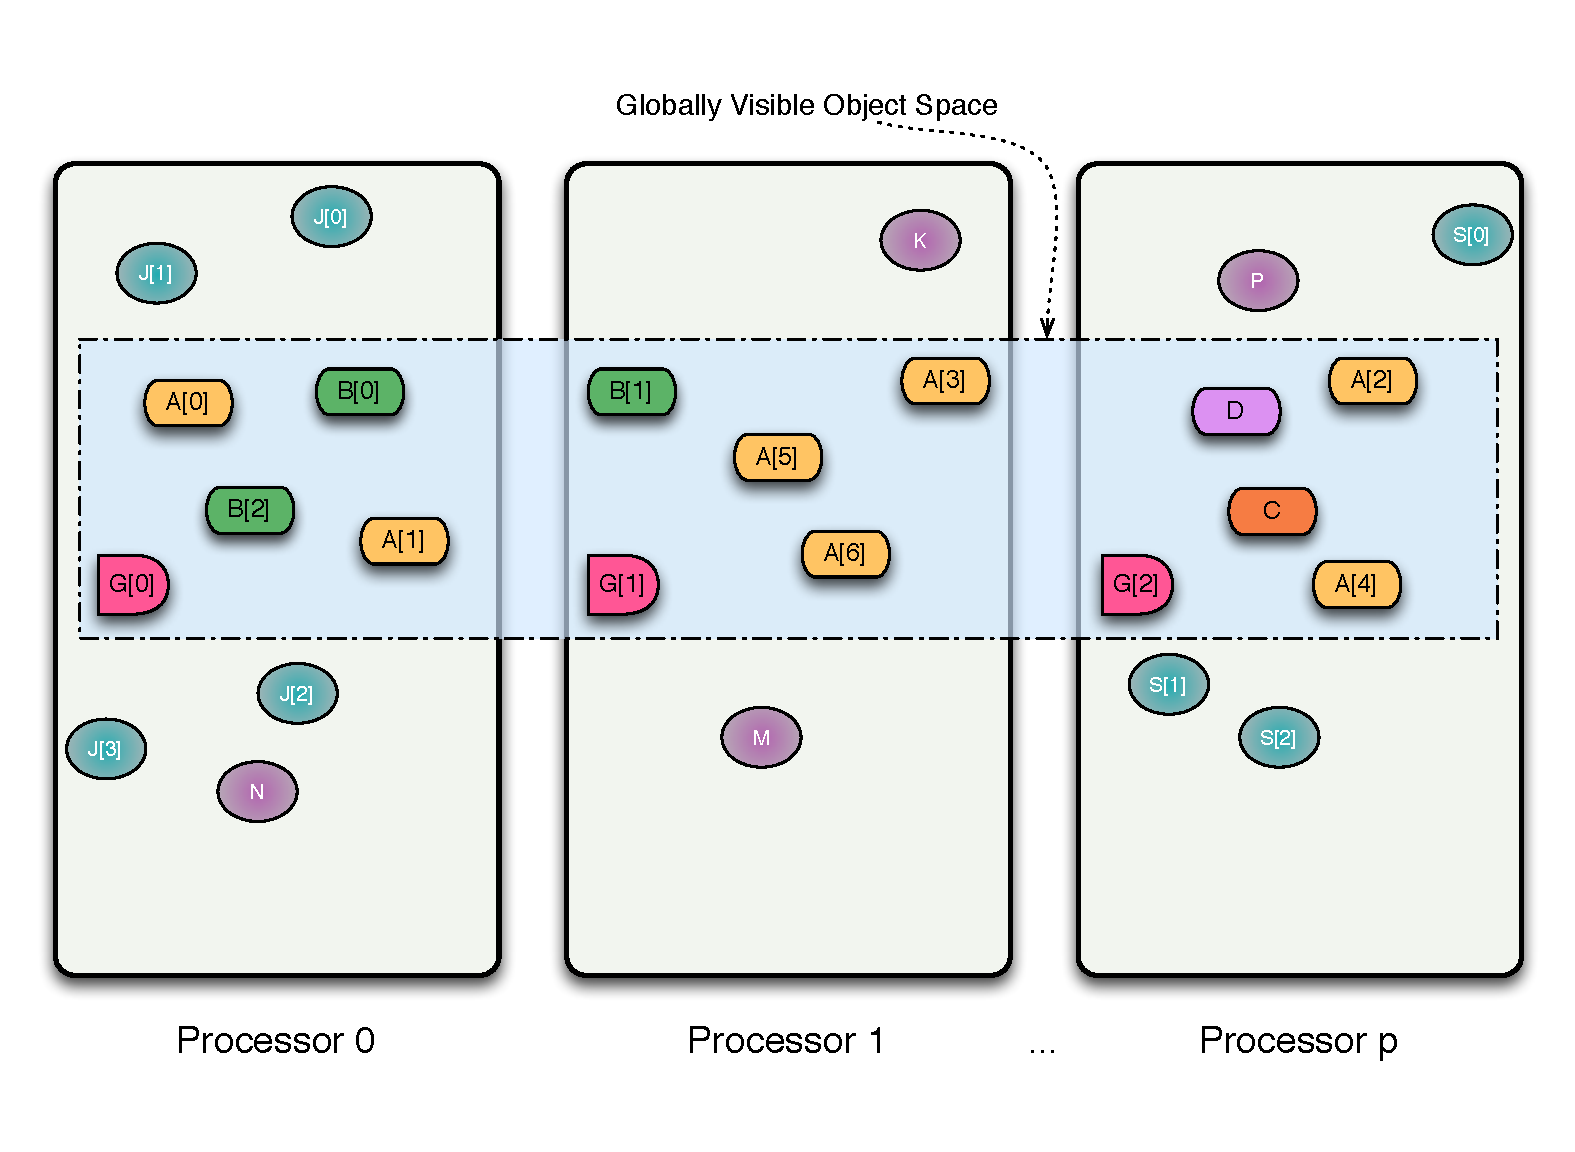
\includegraphics[width=0.9\textwidth]{../figures/progmodel/07-obj-programmer-view.pdf}\end{figure}
\end{frame}


\begin{frame}[fragile,t]
\frametitle{Annotating classes to enable global visibility}
\begin{columns}[t]
\begin{column}{0.4\textwidth}
\begin{block}{In \texttt{foo.ci}}
\begin{lstlisting}
module foo_module {
  array [2D] Foo {
    // . . .
  };
}
\end{lstlisting}
\end{block}
\begin{block}{In \texttt{foo.h}}
\begin{lstlisting}
#include "foo_module.decl.h"

class Foo : public CBase_Foo {
  // . . . 
};
\end{lstlisting}
\end{block}
\end{column}
\begin{column}{0.5\textwidth}
\begin{block}{In \texttt{foo.C}}
\begin{lstlisting}
#include "foo.h"

// . . . 

#include "foo_module.def.h"
\end{lstlisting}
\end{block}
\end{column}
\end{columns}
\end{frame}

\begin{frame}[fragile,t]
\frametitle{Annotating classes to enable global visibility}
\begin{columns}[t]
\begin{column}{0.4\textwidth}
\begin{block}{In \texttt{foo.ci}}
\begin{lstlisting}
module foo_module {
  array [2D] Foo {
    // . . .
  };
}
\end{lstlisting}
\end{block}
\end{column}
\begin{column}{0.5\textwidth}
\begin{block}{In \texttt{foo.C}}
\begin{lstlisting}
#include "foo.h"

// . . . 

#include "foo_module.def.h"
\end{lstlisting}
\end{block}
\end{column}
\end{columns}
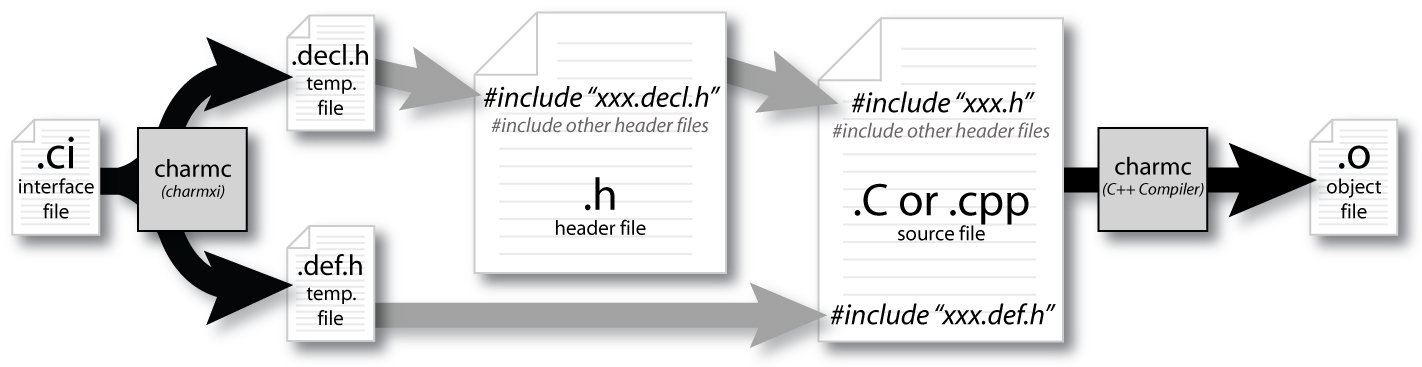
\includegraphics[width=\textwidth]{../figures/charmCompile.jpg}
\end{frame}


\begin{frame}
\frametitle{Indexing into Object Collections}
    \begin{itemize}
       \item multidimensional, integer (1D .. 6D)
        \begin{itemize}
            \item Dense
            \item Sparse
        \end{itemize}
       \item anything hashable (strings, bitvectors)
       \item Static
       \item Dynamic (elements come and go)
    \end{itemize}
\end{frame}


\begin{frame}
\frametitle{Quantum Chemistry: OpenAtom}
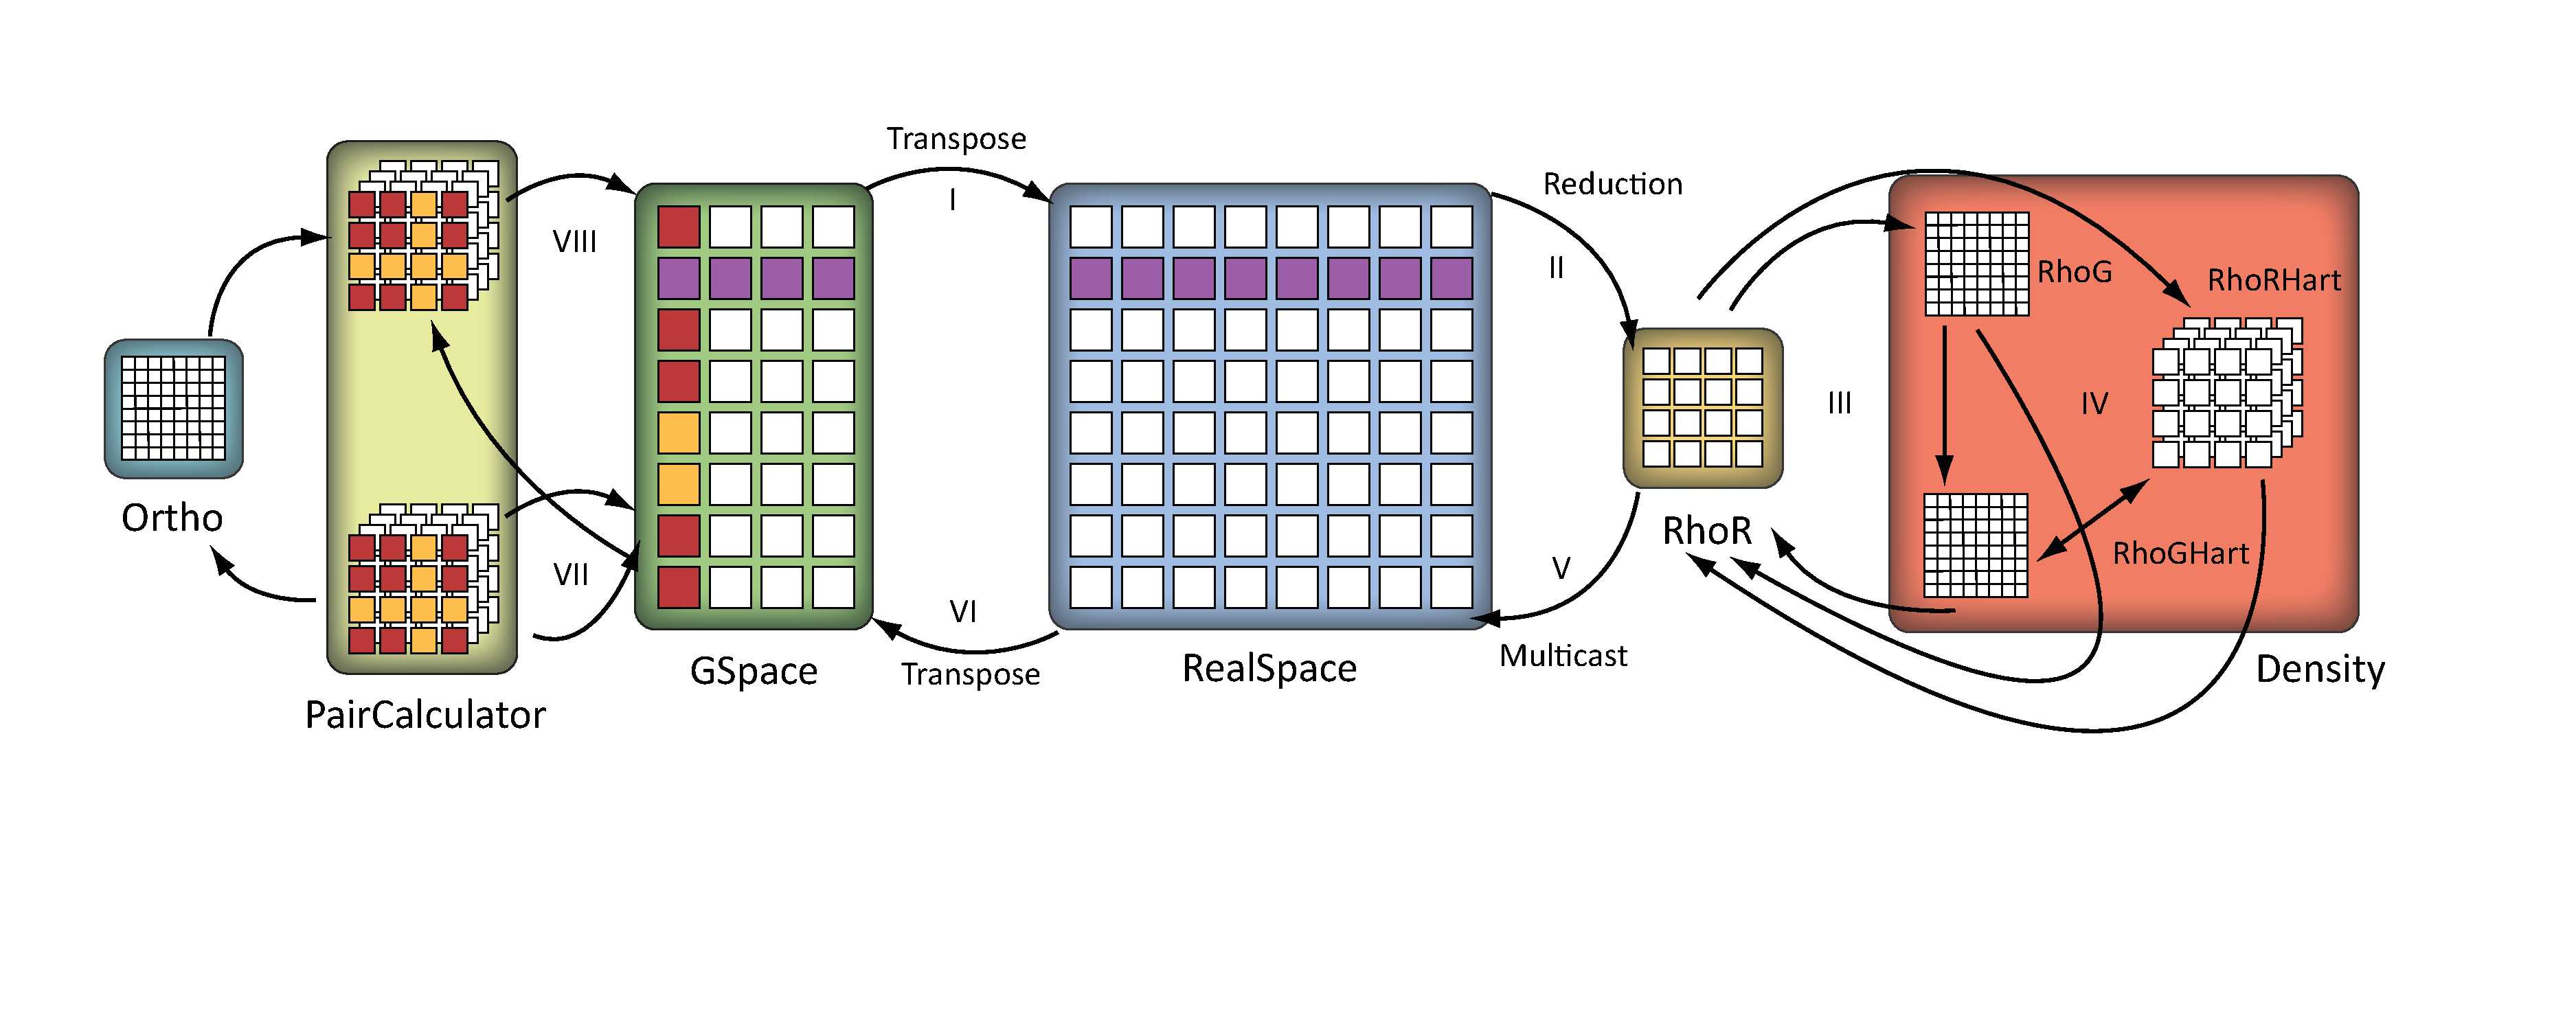
\includegraphics[width=\textwidth]{../figures/openatom/control-flow.pdf}
\end{frame}


\begin{frame}
\frametitle{Quantum Chemistry: OpenAtom}
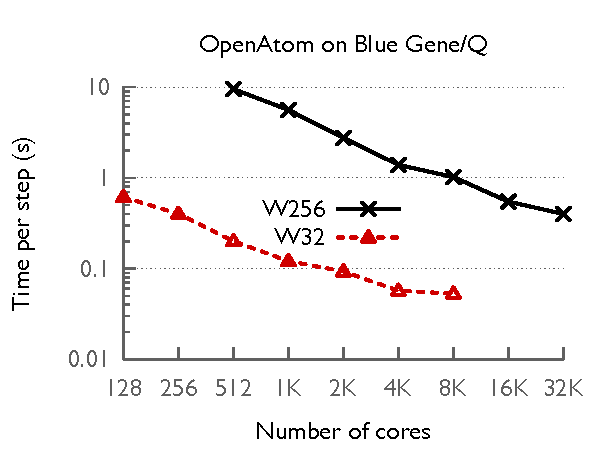
\includegraphics[width=\textwidth]{../figures/openatom/bgq.pdf}
\end{frame}


